\section{Introduction}
\label{sec:intro}
Electron micrographs (Fig.~\ref{fig:img} (a)) are obtained by cryo-electron tomography (CET) \cite{Hawkes2007}, which is an advanced technique to visualize the native environment of neurones, such as cytosol or lysate and lipid membranes~\cite{Lucic2005a}.
%
Among all kinds of cellular materials, biological macromolecules in synaptic cleft regions are one of the hottest study areas, as they play an important role in neurotransmission.
%
In the last decade, it mainly relied on manual segmentation of synaptic cleft regions, which is time-consuming and subjective, to analyze those macromolecules of interest.
%
Our goal in this paper is to develop an automatic approach to accurately extract synaptic cleft regions from noisy electron micrographs (Fig.~\ref{fig:img} (b)).


%The challenges behind this task are not easy to resolve by existing segmentation methods.
Automatic segmentation of synaptic cleft is challenging in many aspects.
Firstly, due to the radiation damaging during CET, electron micrographs suffer from a large amount of noise and low signal-to-noise ratio (SNR).
Secondly, the synaptic cleft region is typically a quite small fraction of a high-resolution $2D$ electron micrograph, which requires a high precision of segmenting small objects.
Thirdly, only the cellular cleft adjacent to one synapse and receiving neurotransmitter molecules from another synapse is the desired synaptic cleft. This requires the segmentation technique to encode much global biological knowledge for judgement.
Finally, as the most of concerned macromolecules exist on the surface of presynaptic membranes, it puts forward a higher demand on accurate contour localization.

\begin{figure}[t]
    \begin{center}
        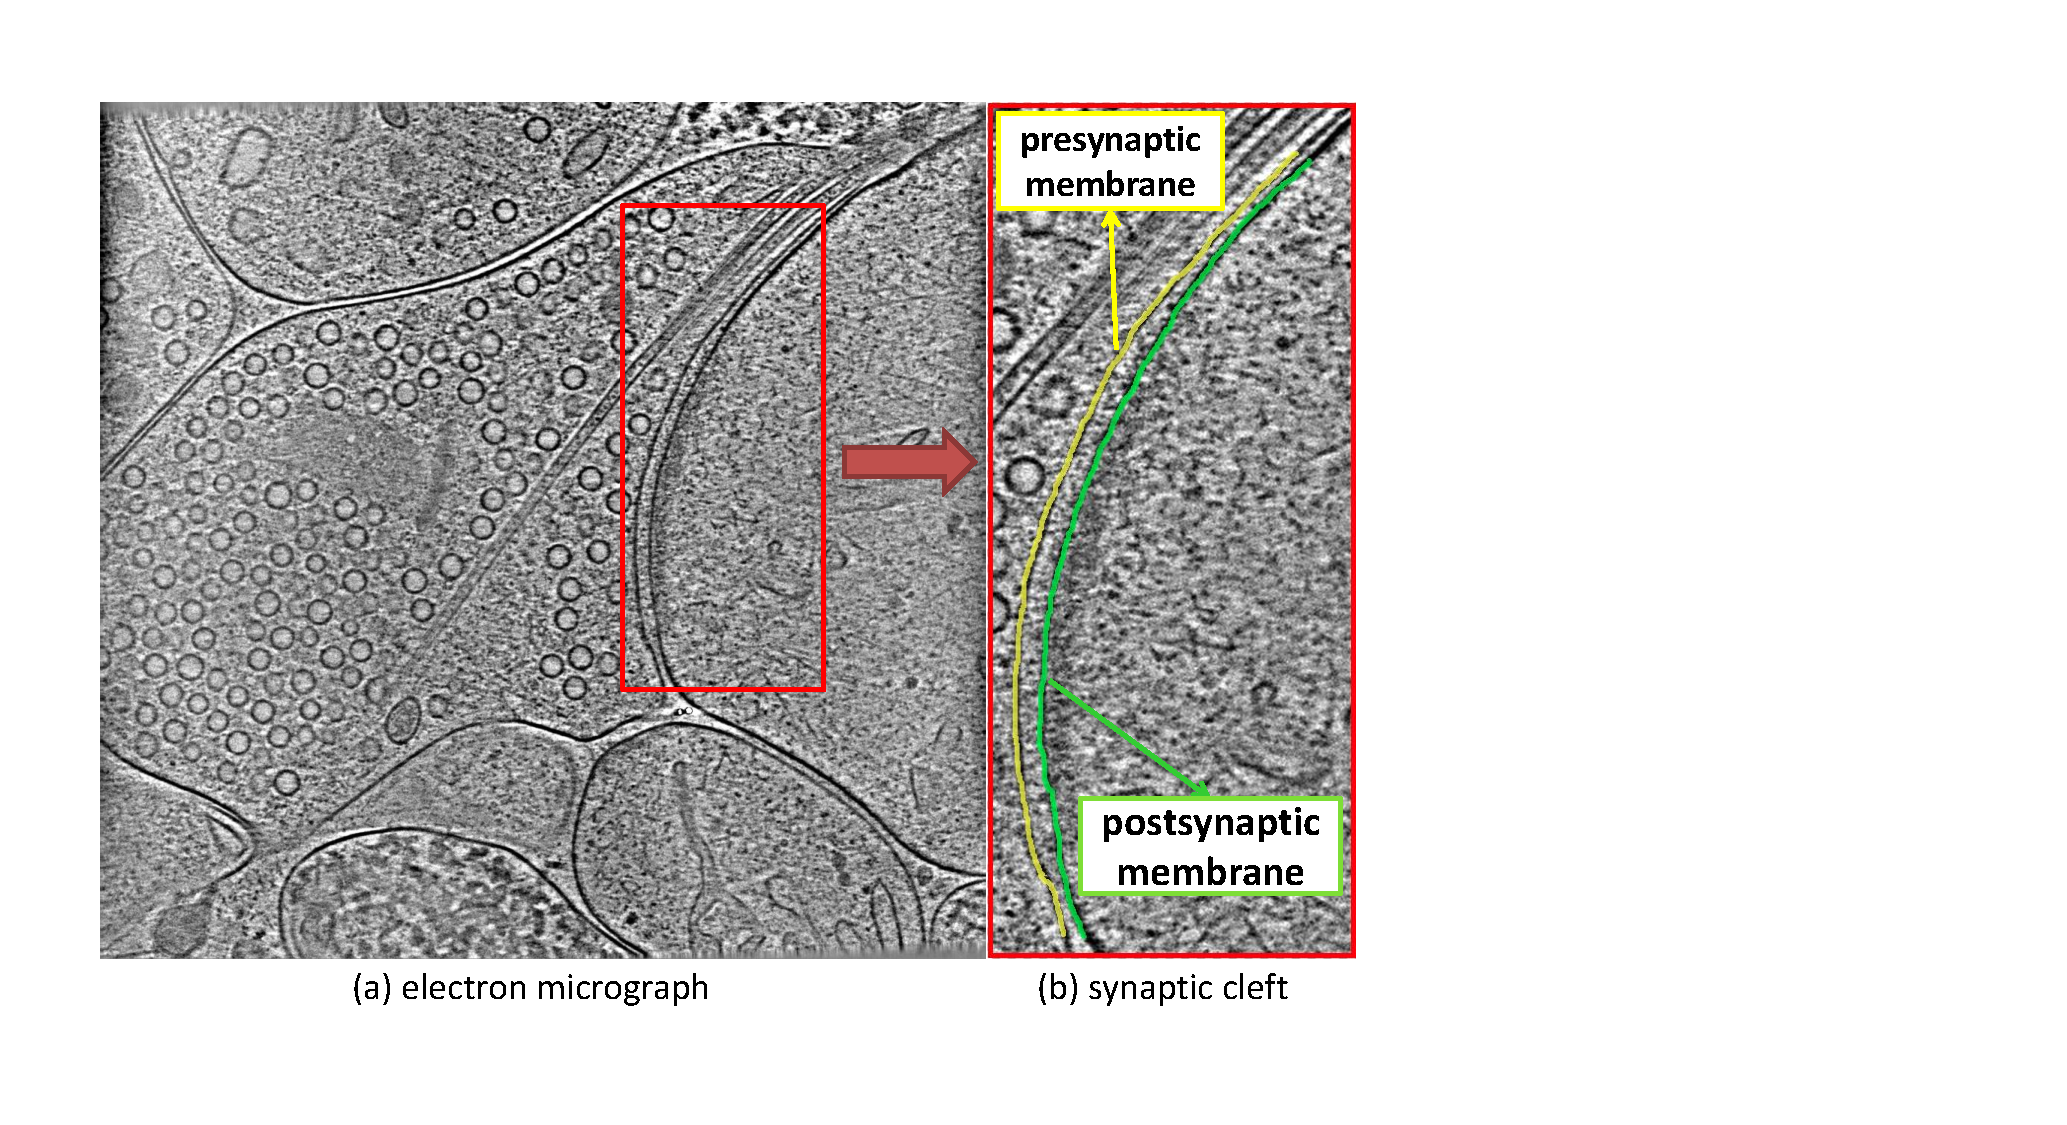
\includegraphics[width=3.4in]{figs/FigImg.pdf}
   \end{center}
\caption{(a) An electron micrograph, where the red box indicates the synaptic cleft region.
            (b) The yellow and green curves are respectively the presynaptic and postsynaptic membranes, which are exactly the contours of a synaptic cleft region.}
\label{fig:img}
\end{figure}

\begin{figure*}[t]
    \begin{center}
        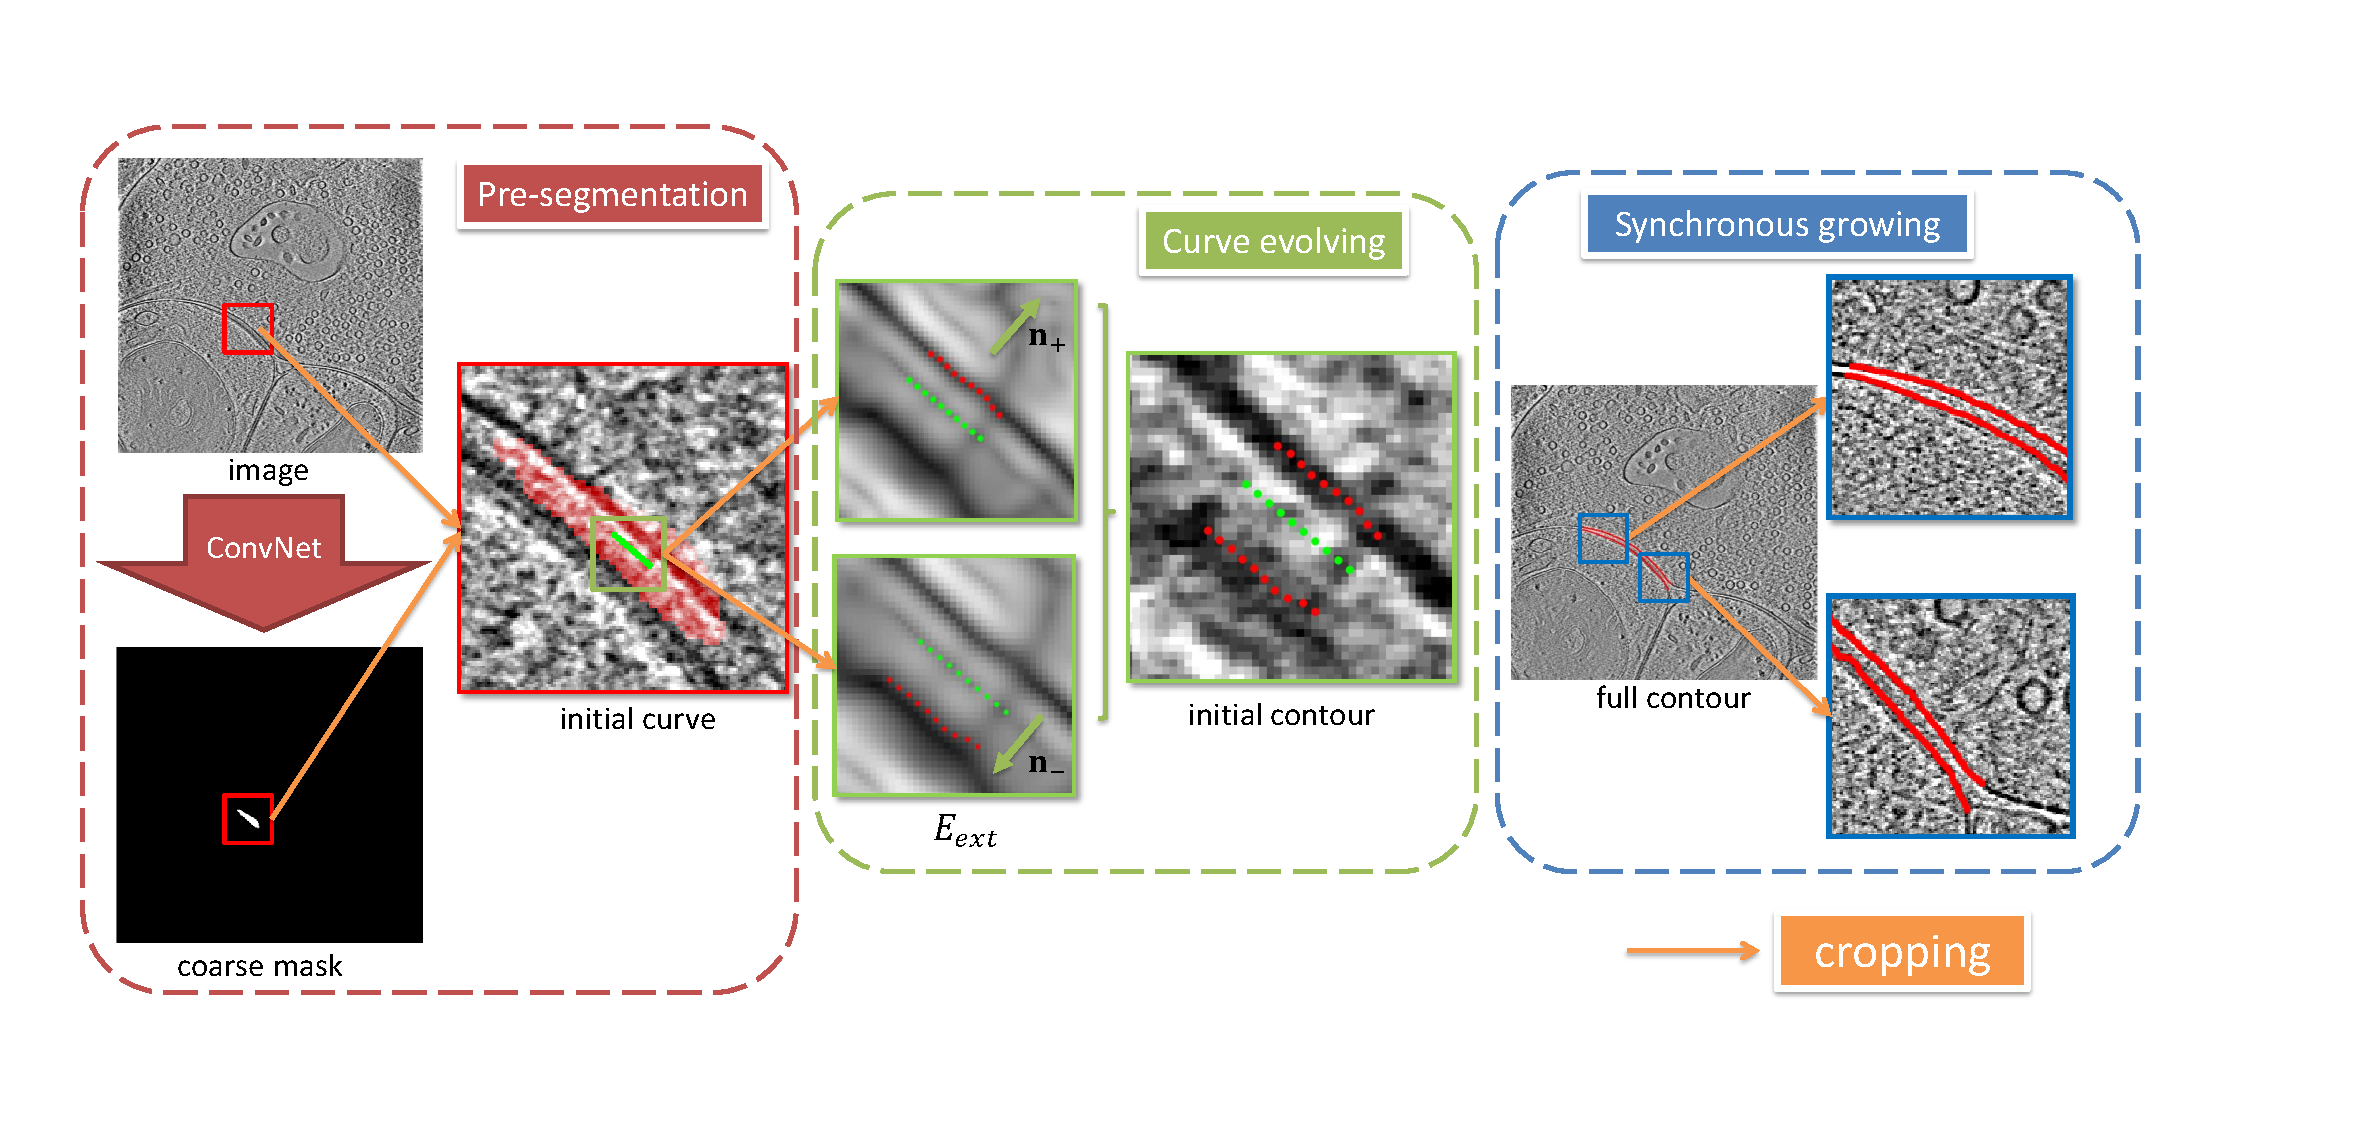
\includegraphics[width=7in]{figs/FigCG.pdf}
   \end{center}
\caption{A brief view of our algorithm in localizing the synaptic cleft region. First a FCN-based model provides a coarse segmentation mask, which can give an initial centric curve (green line) in cleft region.
        Then, the initial curve is respectively evolved along opposite direction ($\mathbf{n}_+$ and $\mathbf{n}_-$) to obtain two pieces of initial contours (red dotted line).
        Finally, the two contours will synchronously grow to localize the whole synaptic cleft region (encircled by red solid curves).}
\label{fig:cg}
\end{figure*}


Recently, fully convolutional networks (FCN)~\cite{Long2015,Ronneberger2015,Chen2016a,Chen2017,Zhao2016} have made a significant process in image segmentation, and variants of FCN \cite{Ronneberger2015,Chen2017,Dhungel2015,Lieman-Sifry2017,Chen2016b,Ourselin} show their promising performance in biomedical image processing.
%
The famous U-net~\cite{Ronneberger2015} directly concatenates the features from downsampling to upsampling layers for the better contour localization.
Soon after, Chen et al.~\cite{Chen2016a} developed the dilated convolution operation by introducing zeros into the original convolutional kernels for larger receptive fields and achieved amazing performance in natural image segmentation.
DCAN~\cite{Chen2017} integrates complementary information of objects and contours in a multi-task learning framework to separate the crowed objects into individual ones.
Moreover, PSPNet~\cite{Zhao2016} uses the more powerful ResNet~\cite{He2016} for feature extracting and proposes a pyramid pooling module to better exploit the global context information.
%
Although these techniques have achieved a great success in many datasets, they still face challenges when processing electron micrographs, which have unique textures and structures.

\comments{
Though FCNs have difficulties on extracting precise boundaries for synaptic cleft, our method is built on FCNs, taking their advantages of efficiently localizing the synaptic cleft region in a large-size electron micrograph.
%
}

%%% remove this part
\comments{
In this paper, we propose an effective framework for segmenting target region in electron micrographs by combining intelligent CNN \xj{{better using FCN?}} and a novel contour growing algorithm.
Our method consists of two main steps.
First, a FCN-based segmentation is employed to coarsely extract the synaptic cleft region. \xj{only one cleft region or mulitple regions?}
%
And then, our contour growing algorithm takes in the segmentation and results in precise contour localizations of target synaptic cleft region.
}
%%%%%%%%%%%%%%% end removing


The insight of our method is that the contours localized by FCNs are usually poor and unsatisfied, due to successive downsampling layers~\cite{Chen2017}, but it successfully produces an accurate localization of our plausible region.
%
Therefore, we utilize the ability of FCN of learning high-level biological knowledge to globally pick out synaptic cleft regions from such a complex environment.
%
Then a novel contour growing process is concatenated to the FCN to extract accurate contours of the target synaptic cleft region.
%

Contour-based method is not brand-new for image segmentation.
Since the active contour was first introduced by Kass et al.~\cite{Kass1988}, it has become one of the most popular tools in contour-based segmentation.
Due to the local and unspecific features used by external tension, much efforts have been made to increase the robustness of active contours.
Cohen et al.~\cite{Cohen1991} added a balloon force as a constant tension to drive the curve away from flat regions.
Xu et al.~\cite{Xu1998} proposed a gradient vector flows method for a larger caption field of external tension.
Leventon et al.~\cite{Leventon2003Statistical} and Tsai et al.~\cite{Tsai2003A} made efforts to employ different regularizing on the curves to make the contour evolution more robust.
Latter, open active contour models have been proposed for medical image analysis, which are designed for extracting tree-shaped structures \cite{Li2009Actin,Xu2013EXTRACTION} by evolving and growing.
Li et al.~\cite{Li2009Actin} introduced the famous stretching open active contour (SOAC) model for extracting actin filaments, by adding non-intensity-adaptive stretching term.
And Xu et al.~\cite{Xu2013EXTRACTION} proposed to extract the clear networks of actin filaments by automatically initializing multiple SOAC models and re-grouping their segmentations.
However, these methods have difficulty on processing the noisy electron micrographs, thus we develop a novel contour growing model for better robustness.

Our contour growing algorithm is robust and efficient, because it is a self-correcting model and uses the local texture information for inference.
With a coarse segmentation of target region, the method first generates a piece of accurate contour using active contour model as origin and then gradually grows the whole contours of the target region.
Especially, as long as the major part of initial curve is successfully evolved to the target contour, the following growing process will be not affected.
%
However, since the contour of a synaptic cleft is not closed and consists of the presynaptic and postsynaptic membranes as shown in Fig.~\ref{fig:img} (b), we should simultaneously grow two piece of contours and decide when the growing terminates according to the distance between these two membranes.


Our main contribution is twofold:
\begin{enumerate}
	\item We propose a new framework to accurately segment the target region in electron micrographs.
	\item A novel updating strategy of active contours is developed, which is more robust and effective for accurate extraction of synaptic regions.
%	\item Specific to segment synaptic cleft region, we propose a algorithm to synchronously grow both two contours.
\end{enumerate}
